

\section{Word learning model}
\label{sec:models}
Latest existing cross-situational models formulate word learning as a
translation problem, where the learner must decide which words in an
utterance correspond to which symbols (or potential referents) in the
perceptual context \citep{yu2007unified,fazly.etal.10csj}. For each new
utterance paired with a symbolic representation of the visual scene,
first the model decides which word is {\it aligned} with which symbol
based on previous associations between the two. Next, it uses the
estimated alignments to update the meaning representation associated
with each word.

We introduce a novel computational model for cross-situational word
learning from captioned images. We reformulate the problem of learning
the meaning of words as a translation problem between words and a {\it
  continuous} representation of the scene; that is, the visual
features extracted from the image. In this setting, the model learns
word representations by taking images and their descriptions one pair
at a time. To learn correspondences between English words and image
features, we borrow and adapt the translation-table estimation
component of the IBM Model 1 \citep{BrownPPM94}. The learning results
in a translation table between words and image-features, i.e.\ a list
of probabilities of image-features given a word.

\subsection{Visual input}
The features of the images are extracted by training a 16-layer
convolutional neural network (CNN) \citep{simonyan2014very} on an
object recognition task.\label{rev:cnndetail}\footnote{We used the F8k
  and F30k features available at
  \url{http://cs.stanford.edu/people/karpathy/deepimagesent/} and the
  data handling utilities from
  \url{https://github.com/karpathy/neuraltalk} for our
  experiments. The pre-trained CNN can be used through the Caffe
  framework \citep{jia2014caffe} and is available at the ModelZoo
  \url{https://github.com/BVLC/caffe/wiki/Model-Zoo}.} The network is
trained to discriminate among 1,000 different object labels on the
ImageNet dataset \citep{deng2009imagenet}. The last layer of the CNN
before the classification layer contains high level visual features of
the images, invariant to particulars such as position, orientation or
size.  We use the activation vector from this layer as a
representation of the visual scene described in the corresponding
caption. Each caption is paired with such a 4,096-dimensional vector
and used as input to a cross-situational word learner.
Figure~\ref{fig:dims} shows three sample images from the F8k
dataset most closely aligned with a particular dimension, as measured
by the cosine similarity between the image and a unit vector parallel
to the dimension axis. For example, dimension 1,000 seems to be related
to water, 2,000 to dogs or perhaps grass, and 3,000 to children.

 \begin{figure}
   \centering
   \begin{tabular}{c|lll}
     {\bf Dimension} & \multicolumn{3}{l}{\bf Top 3 images} \\\hline & & & \\
     1,000
     & 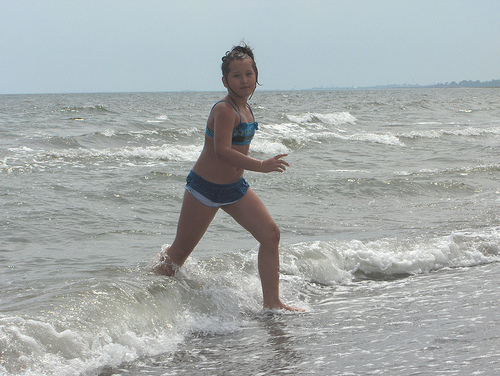
\includegraphics[height=1.5cm]{chapters/TAL/flickr8k/2726262796_03bd63a155.jpg}
     & 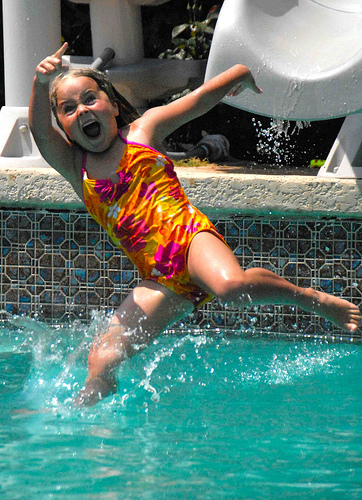
\includegraphics[height=1.5cm]{chapters/TAL/flickr8k/497122685_a51b29dc46.jpg}
     & 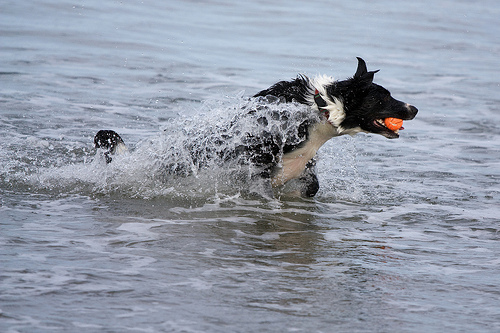
\includegraphics[height=1.5cm]{chapters/TAL/flickr8k/3515904775_f8acc5909e.jpg}
     \\
     & & & \\
     \hline
     & & & \\
     2,000
     & 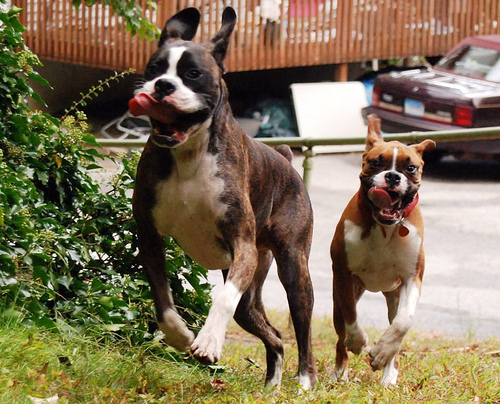
\includegraphics[height=1.5cm]{chapters/TAL/flickr8k/255741044_1102982213.jpg}
     & 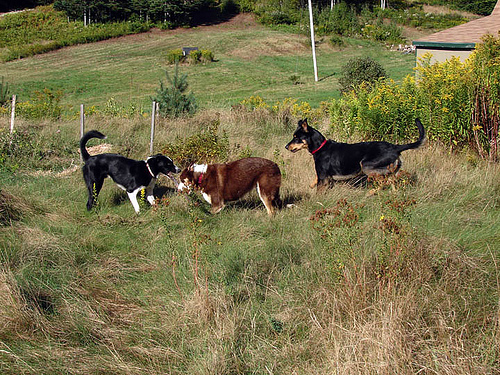
\includegraphics[height=1.5cm]{chapters/TAL/flickr8k/1388970365_162edcceb4.jpg}
     & 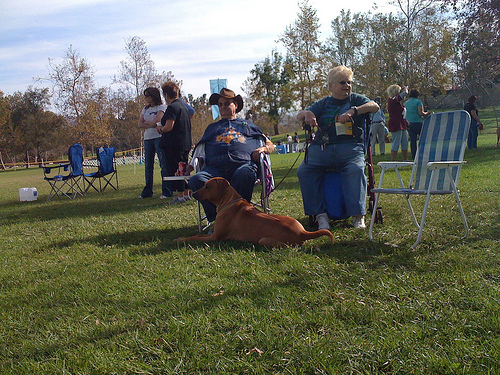
\includegraphics[height=1.5cm]{chapters/TAL/flickr8k/3053813297_7ce5f87710.jpg}
     \\
     & & & \\
     \hline
     & & & \\
     3,000
     & 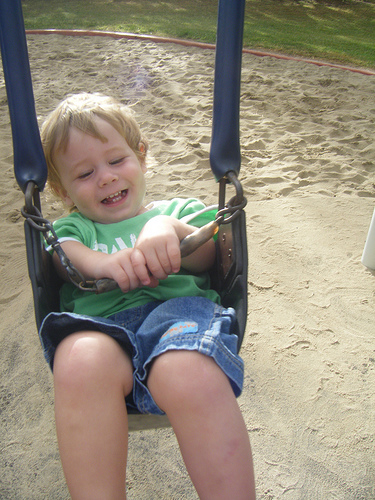
\includegraphics[height=1.5cm]{chapters/TAL/flickr8k/2362481035_a7600875d0.jpg}
     & 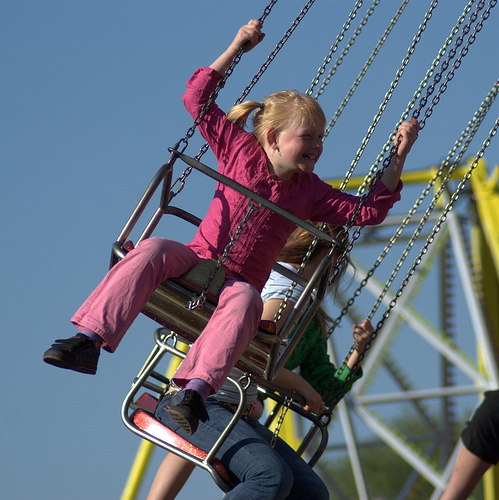
\includegraphics[height=1.5cm]{chapters/TAL/flickr8k/3504940491_94c43792ed.jpg}
     & 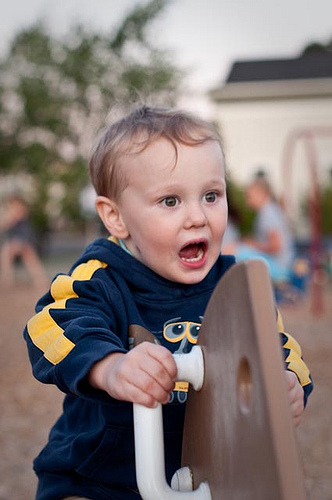
\includegraphics[height=1.5cm]{chapters/TAL/flickr8k/3751594676_edfbfa0688.jpg}
     \\
     & & & \\
     \hline
   \end{tabular}
   \caption{\textit{Dimensions with three most closely aligned images from F8k.}}
   \label{fig:dims}
 \end{figure}


 \subsection{Learning algorithm}
 We adapt the IBM model 1 estimation algorithm in the following
 ways\footnote{The source code for our model is available at
   \url{https://github.com/kadarakos/IBMVisual}.}: (i) like
 \cite{fazly.etal.10csj} we run it in an online fashion, and (ii)
 instead of two sequences of words, our input consists of one sequence
 of words on one side, and a vector of real values representing the
 image on the other side. The dimensions are indexes into the visual
 feature ``vocabulary'', while the values are interpreted as weights
 of these ``vocabulary items''. In order to get an intuitive
 understanding of how the model treats the values in the feature
 vector, we could informally liken these weights to word counts.  As
 an example consider the following input with a sentence and a vector
 of 5 dimensions (i.e.\ 5 features):
\begin{itemize}
\item The blue sky
\item $(2, 0, 2, 1, 0)$
\end{itemize}
Our model treats this equivalently to the following input, with the
values of the dimensions converted to ``feature occurrences'' of each
feature $f_n$.
\begin{itemize}
\item The blue sky
\item $f_1~f_1~f_3~f_3~f_4$
\end{itemize}

The actual values in the image vectors are always non-negative, since
they come from a rectified linear (ReLu) activation. However, they can
be fractional, and thus strictly speaking cannot be literal counts. We
simply treat them as generalized, fractional feature ``counts''.  The
end result is that given the lists of words in the image descriptions
and the corresponding image vectors the model learns a probability
distribution $t(f|w)$ over feature-vector indexes $f$ for every word
$w$ in the descriptions.


\begin{algorithm}
\caption{Sentence-vector alignment model
  (\textsc{Visual})}
\label{algo:ibm-vec}
\begin{algorithmic}[1]
\State { {\bf Input:} visual feature vectors paired with sentences
  $((V_1,S_1),\ldots,(V_N,S_N))$ }
\State { {\bf Output:} translation table $t(f|w)$ }
\State { $D \leftarrow $ dimensionality of feature vectors }
\State { $\epsilon \leftarrow 1$ } \Comment {Smoothing coefficient}
\State { $a[f,w] \leftarrow 0,~ \forall f,w$ } \Comment {Initialize count tables }
\State { $a[\cdot,w] \leftarrow 0,~ \forall w$ }
\State { $t(f|w) \leftarrow \frac{1}{D}$ }
\Comment{ Translation probability $t(f|w)$ }
\For {each input pair (vector $V$, sentence $S$)}
   \For {each feature index $f \in \{1,\ldots,D\}$}
        \State { $Z_f \gets \sum_{w \in S} t(f|w)$ } \Comment { Normalization constant $Z_f$ }
        \For { each word $w$ in sentence $S$}
           \State { $c \gets \frac{1}{Z_f} \times V[f] \times
             t(f|w)$ } \Comment { Expected count $c$ }
           \State { $a[f,w] \gets a[f,w] + c$ }
           \State { $a[\cdot,w] \gets a[\cdot,w] + c$ }
           \Comment { Updates to count tables }
           \State { $t(f|w) \leftarrow \frac{a[f,w]+\epsilon}{a[\cdot,w]+\epsilon D}$ }
           \Comment { Recompute translation probabilities }
\EndFor
\EndFor
\EndFor

\end{algorithmic}
\end{algorithm}

This is our sentence-vector alignment model, \textsc{Visual}. In the
interest of cognitive plausibility, we train it using a single-pass,
online algorithm. Algorithm~\ref{algo:ibm-vec} shows the pseudo-code.
Our input is a sequence of pairs of $D$-dimensional feature vectors
and sentences, and the output is a translation table $t(f|w)$. We
maintain two count tables of expected counts $a[f,w]$ and $a[\cdot,w]$
which are used to incrementally recompute the translation
probabilities $t(f|w)$. The initial translation probabilities are
uniform \mbox{(line 7)}. In lines 12-14 the count tables are updated, based
on translation probabilities weighted by the feature value $V[f]$, and
normalized over all the words in the sentence. In line 15 the
translation table is in turn updated.

\subsection{Baseline models}
\label{sec:baseline}

To asses the quality of the meaning representations learned by our
sentence-vector alignment model \textsc{Visual}, we compare its
performance in a set of tasks to the following baselines:
\begin{itemize}
  \item \textsc{Monoling:} instead of aligning each sentence with its
    corresponding visual vector, this variation aligns two copies of
    each sentence with each other, and thus learns word
    representations based on word-word co-occurrences\footnote{This
      model does not estimate probabilities of translation of a word
      to itself, that is probabilities of the form $t(w|w)$.}.
  \item \textsc{Word2Vec:} for comparison we also report results with the skip-gram embedding model, also known as \textsc{word2vec} which builds word
    representations based on word-word co-occurrences as well
    \citep{mikolov2013efficient,mikolov2013distributed}. \textsc{Word2vec}
    learns a vector representation (embedding) of a word which
    maximizes performance on predicting words in a small window around
    it.
\end{itemize}
